\section{Normal Situation} %5.1

Applying data sets which contains features for prediction (mentioned in Section \ref{sec:normal-predic}), the Arctic Sea Ice Extent variation in 10 years (from 2021 to 2030) was plotted (Figure \ref{4.3.1-10yrs}).

\begin{figure}[htbp]
\centering
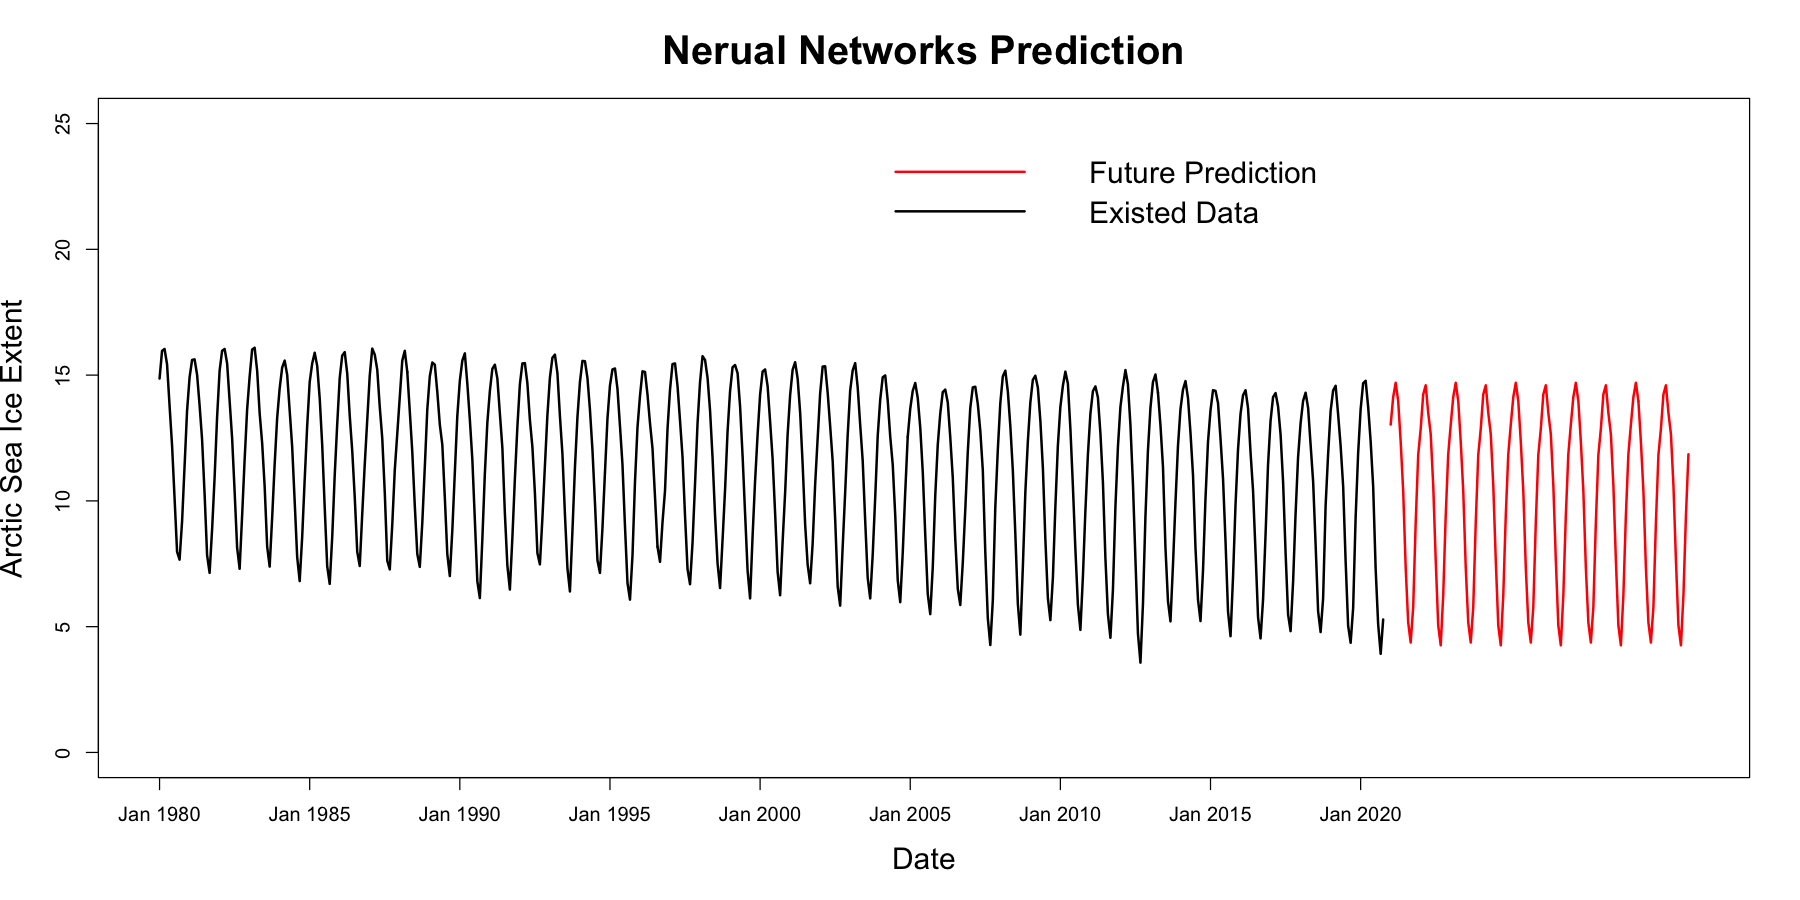
\includegraphics[width = 1.0\textwidth]{Figure/4.3.1-10yrs.png}
\caption{Future prediction of Arctic sea ice: 10 years' normal situation prediction ---- monthly.}
\label{4.3.1-10yrs}
\end{figure}


As the monthly figure (Figure \ref{4.3.1-Normal-Prediction}) shown, the sea ice extent fluctuation conforms to the expected seasonality and continues the main trend. Therefore, we can conclude that the prediction based on the neural network and the prediction data set is reasonable.

\begin{figure}[htbp]
\centering
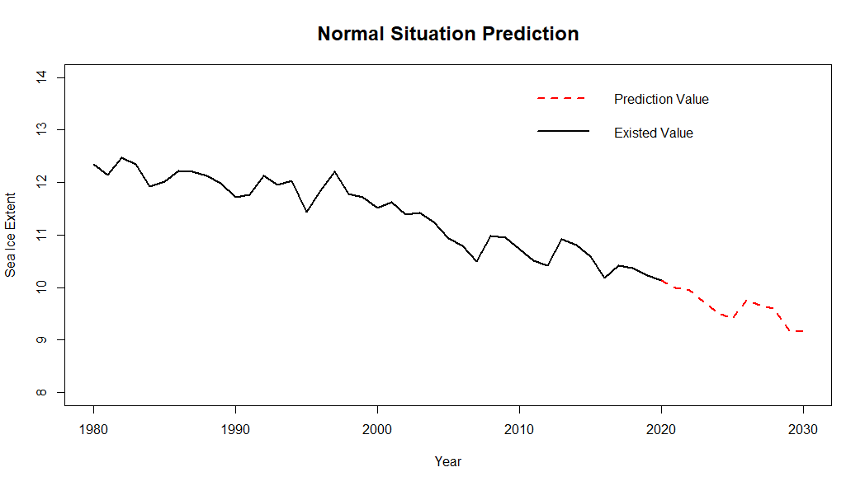
\includegraphics[width = 1.0\textwidth]{Figure/4.3.1-Normal-Prediction.png}
\caption{Future prediction of Arctic sea ice: 50 years' normal situation prediction.}
\label{4.3.1-Normal-Prediction}
\end{figure}

To predict a long-term trend, it is more intuitive to visualize using annual average. Based on Random Forest model, the Arctic sea ice extent decreased from 10.00 $\text{Mkm}^2$ in 2020 to 9.41 $\text{Mkm}^2$ in 2030, reducing by 5.9\%.

\newpage